\section{Results}

\subsection{Dataset 1: \texttt{robotdata1.log}}

Figure~\ref{fig:Screenshot-video_log1-10k_good} shows snapshots from a run using the first data log. The particles start spread across the map but are able to converge to a single cluster in a reasonable amount of time. The motion of this cluster, including changing directions twice in the hallway and ending in the room, is consistent with \texttt{robotmovie1.gif}, indicating the particle filter was able to accurately localize the robot. Total runtime was around 25 minutes.\\ Video is available here: \url{https://www.youtube.com/watch?v=DxhAmjijvzI}

\begin{figure}[h]
\centering
\begin{subfigure}[b]{0.49\textwidth}
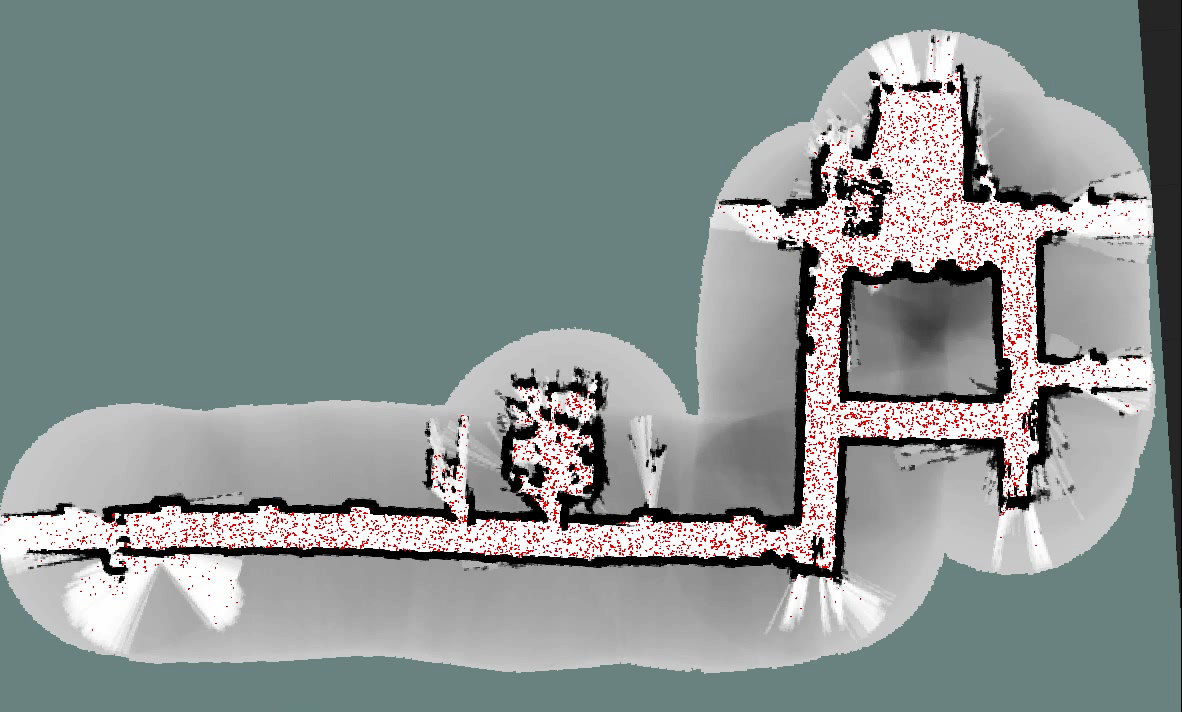
\includegraphics[width=\linewidth]{figures/Screenshot-video_log1-10k_good-1}
\caption{Initial distribution of particles}
\label{fig:Screenshot-video_log1-10k_good-1}
\end{subfigure}
\begin{subfigure}[b]{0.49\textwidth}
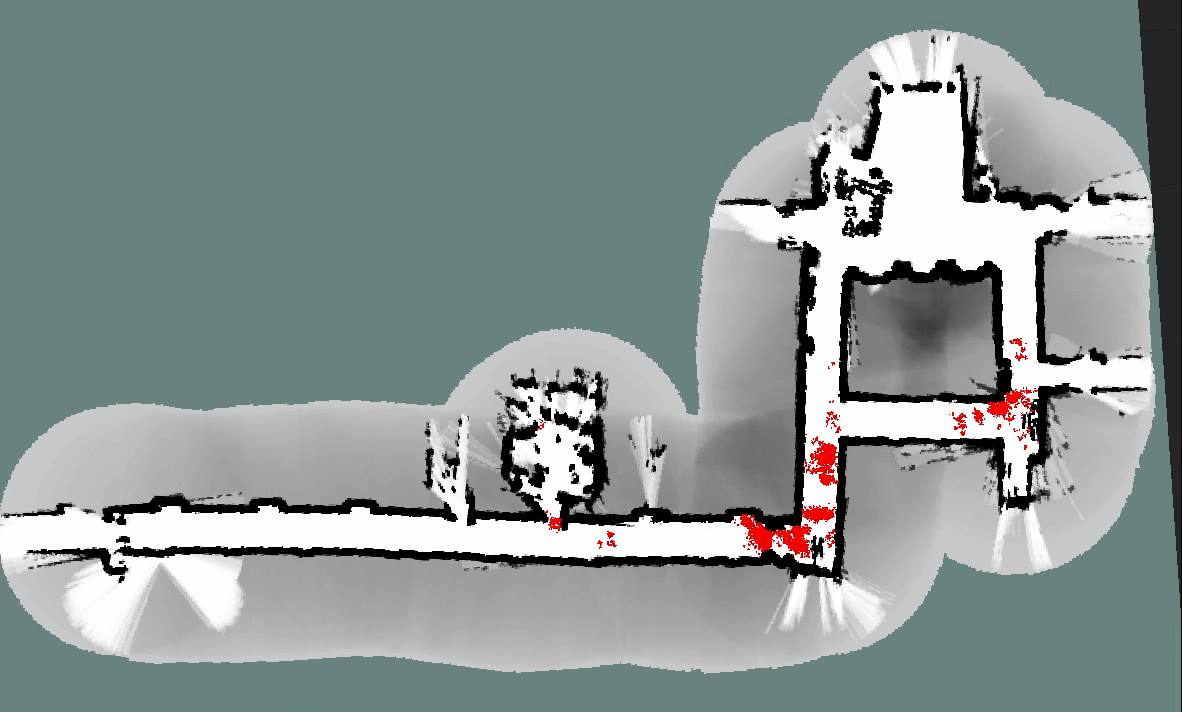
\includegraphics[width=\linewidth]{figures/Screenshot-video_log1-10k_good-2}
\caption{Particles start to converge}
\label{fig:Screenshot-video_log1-10k_good-2}
\end{subfigure}
\\
\begin{subfigure}[b]{0.49\textwidth}
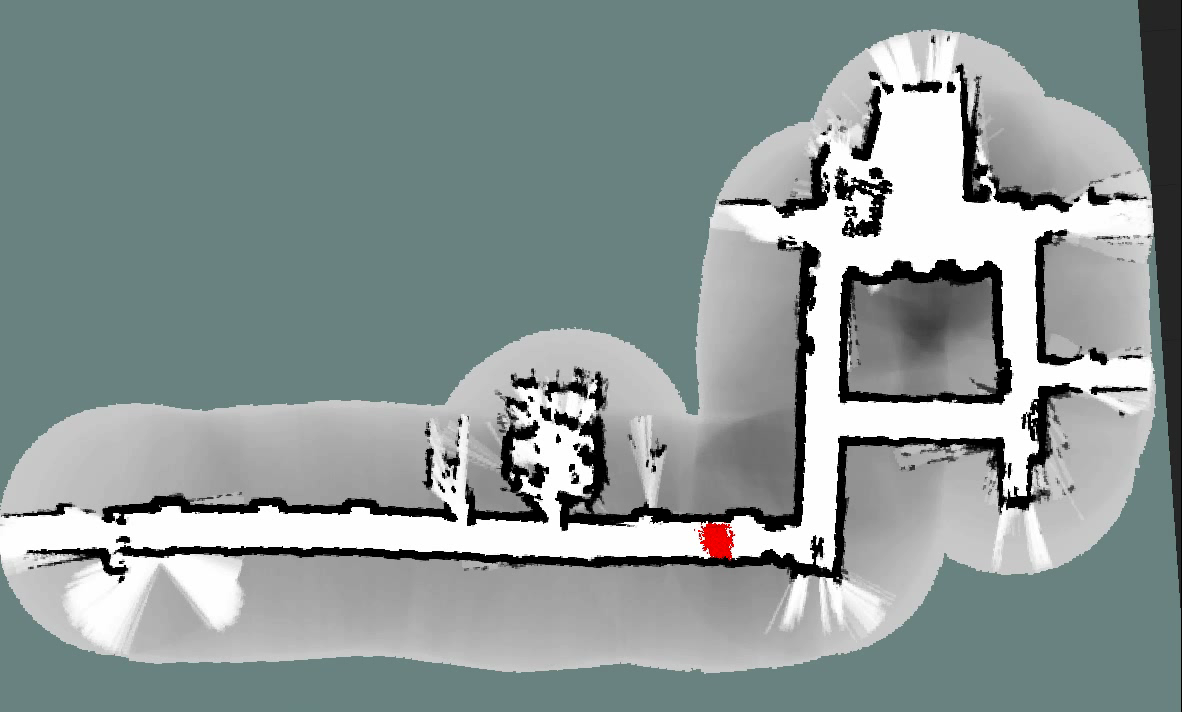
\includegraphics[width=\linewidth]{figures/Screenshot-video_log1-10k_good-3}
\caption{Particles have converged to one location}
\label{fig:Screenshot-video_log1-10k_good-3}
\end{subfigure}
\begin{subfigure}[b]{0.49\textwidth}
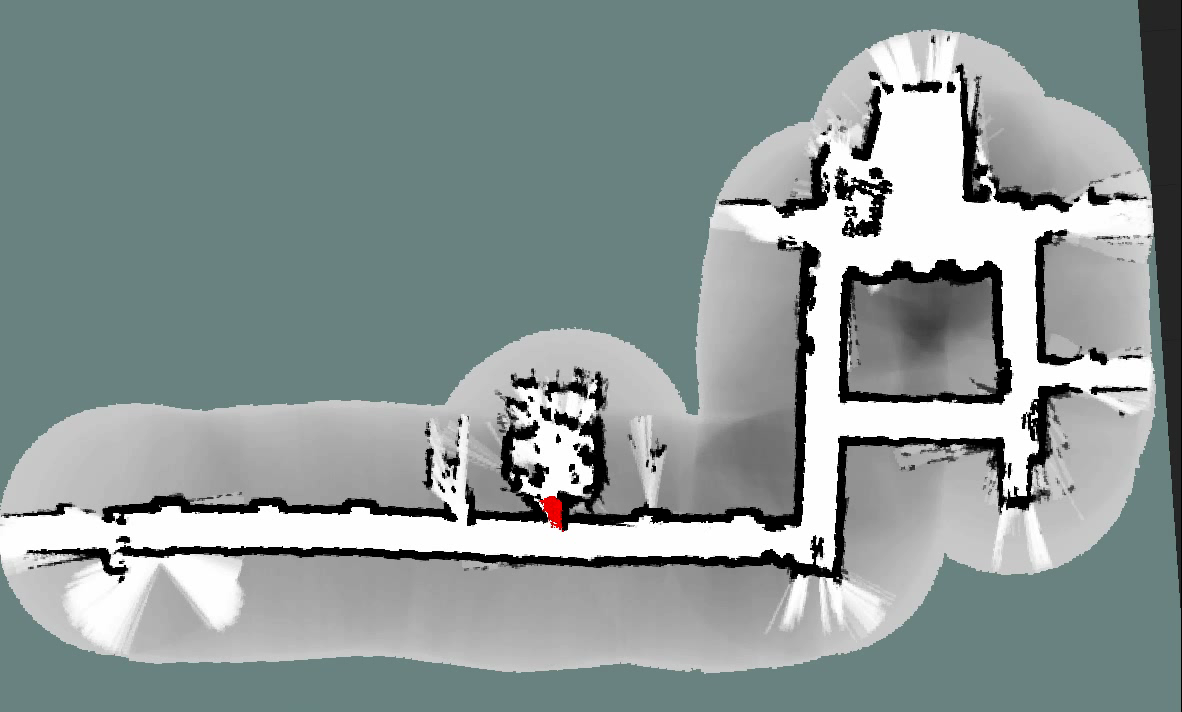
\includegraphics[width=\linewidth]{figures/Screenshot-video_log1-10k_good-4}
\caption{Particles finish inside the room, as expected}
\label{fig:Screenshot-video_log1-10k_good-4}
\end{subfigure}
\caption{Snapshots from \texttt{robotdata1.log} showing particles converging to the long hallway, turning around at the end, and entering the room.
\label{fig:Screenshot-video_log1-10k_good}}
\end{figure}



\subsection{Dataset 2: \texttt{ascii-robotdata5.log}}

Figure~\ref{fig:Screenshot-video_log5-10k_goodenough} shows a few snapshots from a run using the fifth data log. Again, the particles converge to one cluster reasonably quickly and traverse the hallway. However, we noticed the cluster seems to overshoot when making the turn, leading to many particles being constrained by the wall, and consequently down-weighted. This problem seems to resolve itself though, as the particles are able to complete the turn. Though there was no ground truth provided for this set, the motion of the final cluster of particles seems to be consistent with the odometry data (Fig.~\ref{fig:log5odom}). Total runtime was around 35 minutes.\\
Video is available here:  \url{https://www.youtube.com/watch?v=AgGZ6cR-dyk}


\begin{figure}
\centering
\begin{subfigure}[b]{0.49\textwidth}
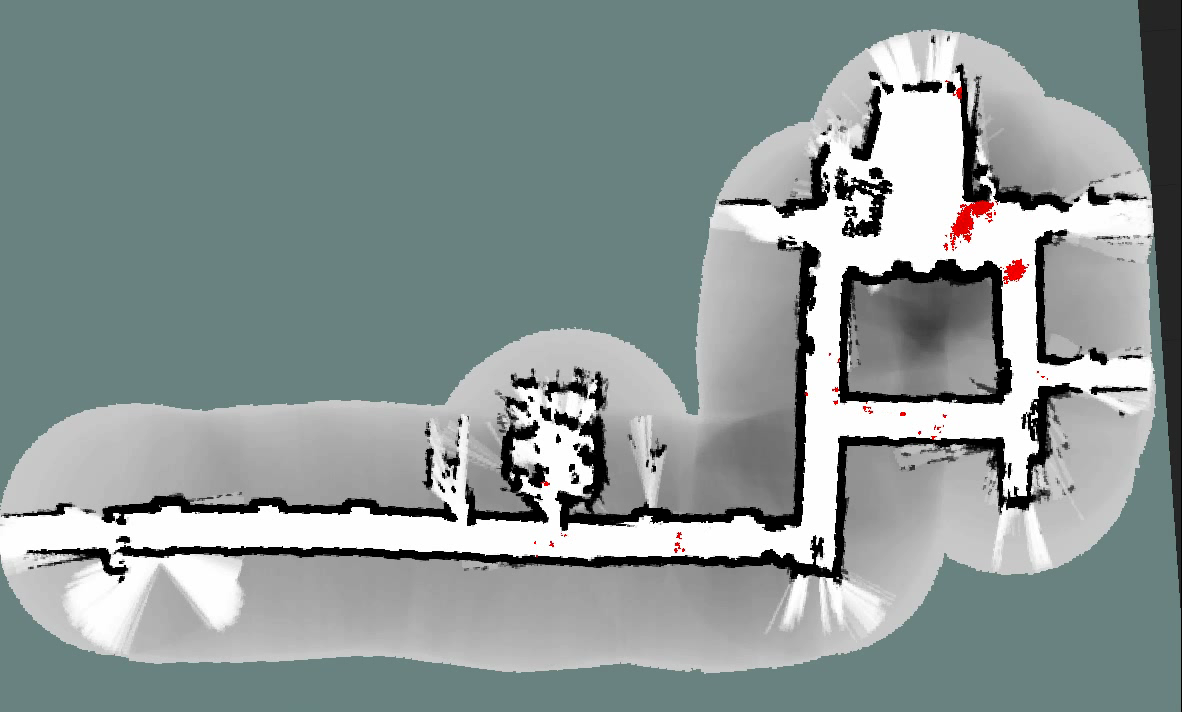
\includegraphics[width=\linewidth]{figures/Screenshot-video_log5-10k_goodenough-1}
\caption{Particles start converging to two large clusters}
\label{fig:Screenshot-video_log5-10k_goodenough-1}
\end{subfigure}
\begin{subfigure}[b]{0.49\textwidth}
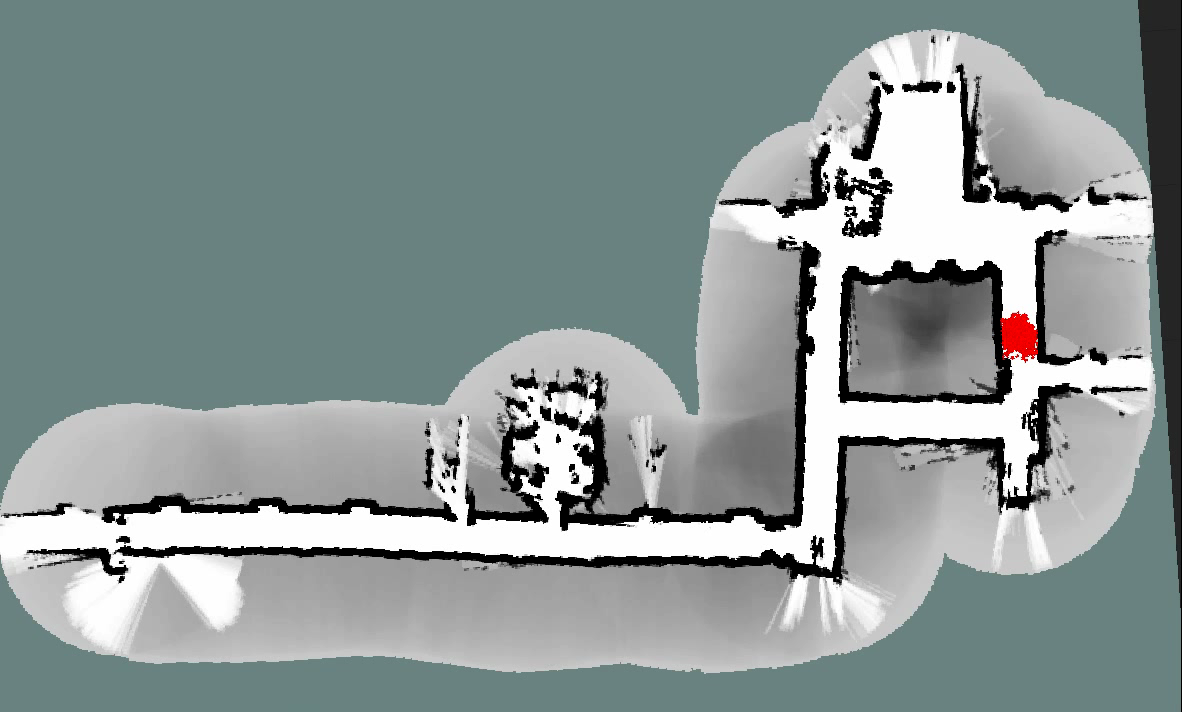
\includegraphics[width=\linewidth]{figures/Screenshot-video_log5-10k_goodenough-2}
\caption{Second cluster dominates}
\label{fig:Screenshot-video_log5-10k_goodenough-2}
\end{subfigure}
\\
\begin{subfigure}[b]{0.49\textwidth}
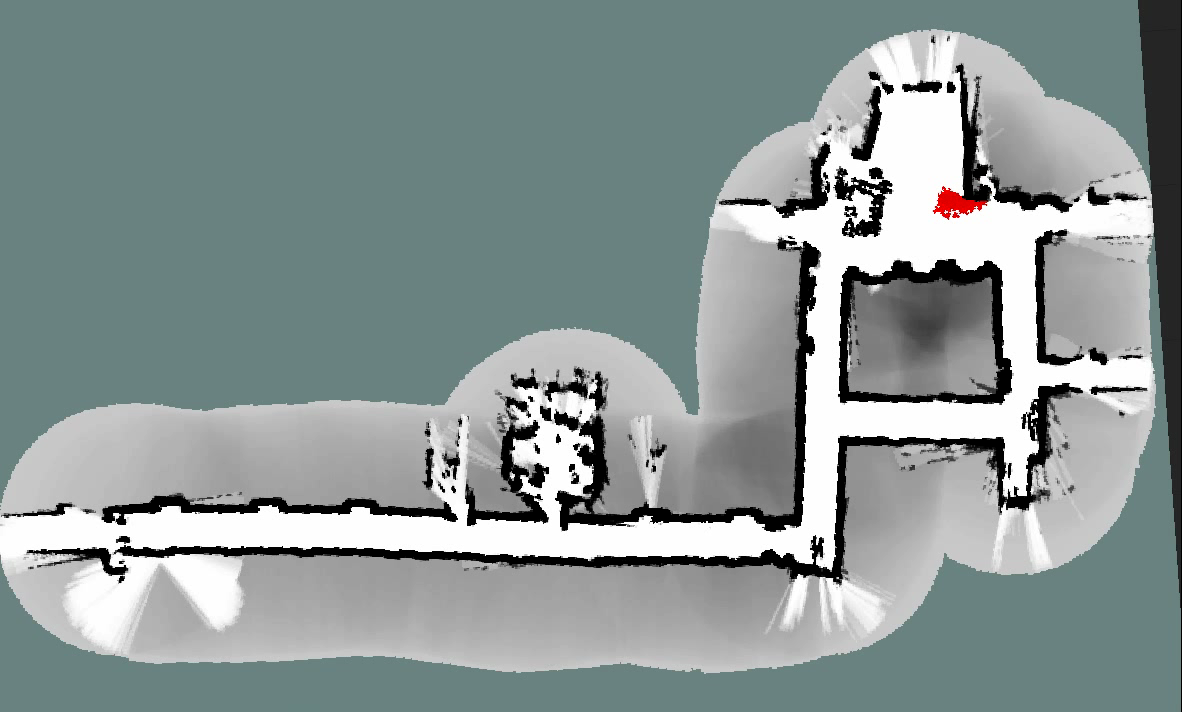
\includegraphics[width=\linewidth]{figures/Screenshot-video_log5-10k_goodenough-3}
\caption{Particles turning left into the open area but seem slightly off}
\label{fig:Screenshot-video_log5-10k_goodenough-3}
\end{subfigure}
\begin{subfigure}[b]{0.49\textwidth}
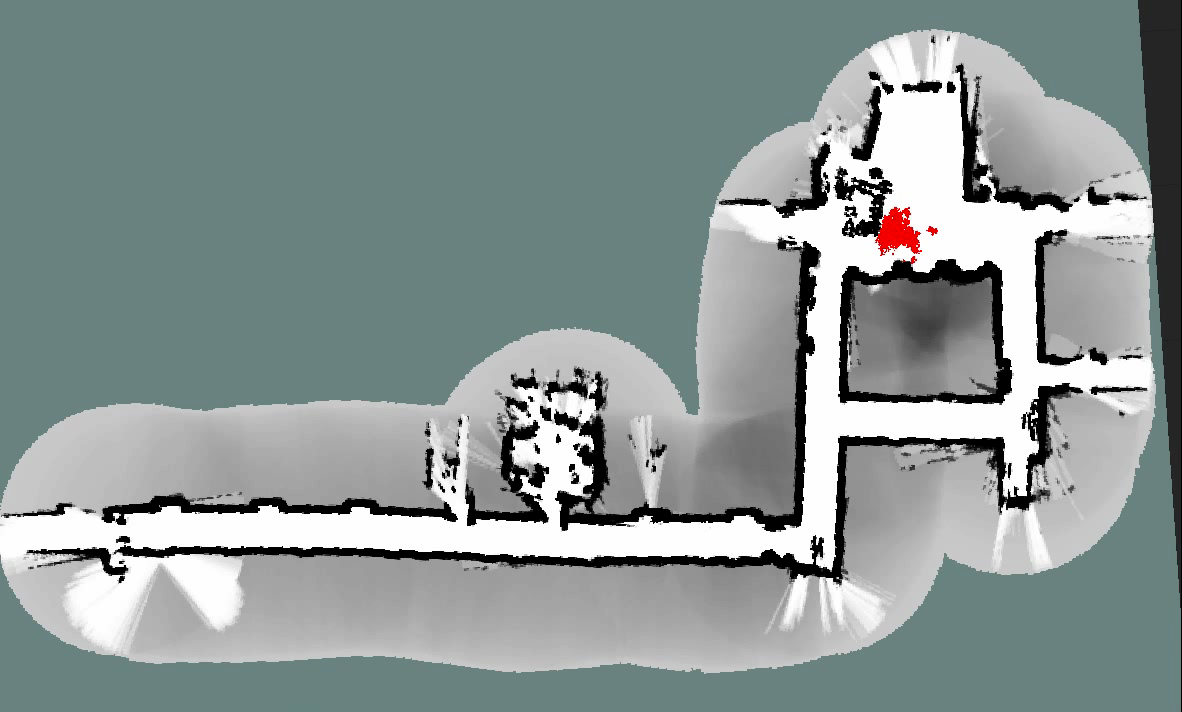
\includegraphics[width=\linewidth]{figures/Screenshot-video_log5-10k_goodenough-4}
\caption{Particles complete the left turn and stop}
\label{fig:Screenshot-video_log5-10k_goodenough-4}
\end{subfigure}
\caption{Snapshots from \texttt{ascii-robotdata5.log} showing particles converging to the hallway on the right, turning around partway through, and turning left into the open area at the top.
\label{fig:Screenshot-video_log5-10k_goodenough}}
\end{figure}

\begin{figure}
\centering
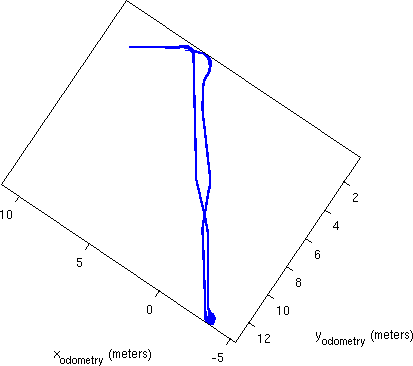
\includegraphics[width=0.45\linewidth]{figures/log5odom}
\caption{Odometry data from \texttt{ascii-robotdata5.log}}
\label{fig:log5odom}
\end{figure}
